\section{Verifying calibration}
\label{sec:verifying_calibration}

\newcommand{\pluginEst}[0]{\ensuremath{\hat{E}_{\textup{pl}}^2}}
\newcommand{\cancelEst}[0]{\ensuremath{\hat{E}^2}}
\newcommand{\ltwoerror}[0]{\ensuremath{{\hat{E}^*}^2}}
\newcommand{\piSmallBound}[0]{\ensuremath{\frac{12}{n}\log{\frac{2B}{\delta}}}}

\tm{I wonder we should have subscript for $\cancelEst$. $\ensuremath{\hat{E}_{\textup{cxl}}^2}$? Sounds a bit verbose..}
Before deploying our model we would like to check that it has calibration error below some desired threshold $\epsilon^2$. In this section we show that we can efficiently estimate the calibration error of binned models, if the binning scheme is 2-well-balanced. Recent work in machine learning typically estimates each term in the calibration error directly from samples~\cite{nguyen2015posterior, hendrycks2019anomaly, kuleshov2015calibrated, hendrycks2019pretraining}. Older work in meteorology~\cite{brocker2012empirical, ferro2012bias} notices that this leads to a biased estimate, and proposes a `debiased' estimator that subtracts off an approximate correction term to reduce the bias. Our contribution is to show that while the naive estimator requires samples proportional to $B$ to estimate the calibration error, the debiased estimator requires samples proportional to $\sqrt{B}$. To our knowledge we are the first to show an \emph{improved sample complexity}---prior work only showed that the naive estimator is biased.

Suppose we wish to measure the calibration error of a model $f : \mathcal{X} \to S$ where $S \subseteq [0, 1]$ and $|S| = B$. Suppose we get an evaluation set $T_n = \{(x_1, y_1), \dots, (x_n, y_n)\}$. Past work typically estimates the calibration error by directly estimating each term from samples:

\begin{restatable}[Plugin estimator]{definition}{pluginDfn}
\label{dfn:plugin-estimator}
  Let $L_s$ denote the $y_j$ values where the model outputs $s$: $L_s = \{ y_j \; | \; (x_j, y_j) \in T_n\wedge f(x_j) = s \}$. Let $\hat{p}_s$ be the estimated probability of $f$ outputting $s$:
$\hat{p}_s = \frac{|L_s|}{n}$.

Let $\hat y_i$ be the empirical average of $Y$ when the model outputs $s$: $\hat y_s = \sum_{y \in L_s} \frac{y}{|L_s|}$

  The plugin estimate for the $\ell_2^2$ calibration error is \tm{$\ell^2$ calibration error sounds clearer}the weighted squared difference between $\hat y_s$ and $s$:
\[ \pluginEst{} = \sum_{s \in S} \hat{p}_s (s - \hat y_s)^2 \]
\end{restatable}
\pl{can we just use $L^2$ for this whole paper?}

Alternatively, \cite{brocker2012empirical, ferro2012bias} propose to subtract an approximation of the bias from the estimate:

\begin{restatable}[Debiased estimator]{definition}{cancelingDfn}
  The debiased estimator for the $\ell_2^2$ error is:
\[ \hat{E}^2 = \sum_{s \in S} \hat{p}_s \Big[ (s - \hat{y}_s)^2 - \frac{\hat{y}_s(1 - \hat{y}_s)}{\hat{p}_sn-1} \Big] \]
\end{restatable}

We are interested in analyzing the number of samples required to estimate the calibration error within a constant multiplicative factor, that is to give an estimate $\hat{E}^2$ such that $\lvert \hat{E}^2 - {E^*}^2 \rvert \leq \frac{1}{2}{E^*}^2$ (where $\frac{1}{2}$ can be replaced by any constant $r$ with $0 < r < 1$). Our main result is that the plugin estimator requires $\widetilde{O}(\frac{B}{\epsilon^2})$ samples (Theorem~\ref{thm:final-plugin}) while the debiased estimator requires $\widetilde{O}(\frac{\sqrt{B}}{\epsilon^2})$ samples (Theorem~\ref{thm:final-ours}), where $\epsilon = {E^*}^2$.


% Suppose we want to check if our model has calibration error $\leq \epsilon^2$. With high probability, if the calibration error is $> \epsilon^2$, we should output that the model is not calibrated, but if the calibration error is $\leq \frac{1}{2} \epsilon^2$, we should output that it is calibrated. They way we do this is we take $n$ samples and get an estimate, $\hat{E}^2$, of the calibration error---we output `calibrated' iff $\hat{E}^2 \leq \frac{3}{4} \epsilon^2$. We are interested in analyzing how large $n$ needs to be. Equivalently, we can examine the number of samples required to estimate the calibration error within a constant multiplicative factor, that is $\lvert \hat{E}^2 - {E^*}^2 \rvert \leq \frac{1}{2}{E^*}^2$.

% Concretely, suppose we are interested in checking if our model has calibration error $\leq \epsilon$
% \pl{but this is not what we actually show due to $r$}. If the calibration error is $> \epsilon$, then with high probability we should output that it is not calibrated \pl{be more precise}\ak{Which part should be more precise?}
% \pl{what does saying 'it's calibrated' mean? I think you mean calibration error
% less than $\epsilon$; I think you want to say, the contract is: fix an
% $\epsilon$; we want to do a hypothesis test of whether this error is $< r \epsilon$ or $> \epsilon$; basically the contract is not clear}.
% If the calibration error is $< r\epsilon$, where $0 < r < 1$ is a user-specified effect size, then with high probability we should output that the model is calibrated.


% Our main result is that to check if the $\ell_2^2$ calibration error is $\leq \epsilon^2$, the plugin estimator requires $\widetilde{O}(\frac{B}{\epsilon^2})$ samples (Theorem~\ref{thm:final-plugin}) while the debiased estimator requires $\widetilde{O}(\frac{\sqrt{B}}{\epsilon^2})$ samples (Theorem~\ref{thm:final-ours}):

\begin{restatable}[Plugin bound]{theorem}{finalPlugin}
\label{thm:final-plugin}
  Suppose we have a binned model with $\ell_2^2$ calibration error ${E^*}^2 = \epsilon^2$, where the binning scheme is 2-well-balanced, that is $\forall i.\;p_i \geq \frac{1}{2B}$. If $n \geq c\frac{B}{\epsilon^2}\log{\frac{B}{\delta}}$ for some universal constant $c$ then for the plugin estimator: $\frac{1}{2} {E^*}^2 \leq \pluginEst{} \leq \frac{3}{2} {E^*}^2$ with probability at least $1 - \delta$.
 % Suppose we have a binned model with $\ell_2^2$ calibration error ${E^*}^2 = \epsilon^2$, where the binning scheme is 2-well-balanced, that is $\forall i.\;p_i \geq \frac{1}{2B}$, and $n = \widetilde{O}(\frac{B}{\epsilon^2})$ where $\widetilde{O}$ hides $\log$ factors. Then for the plugin estimator: $\frac{1}{2} {E^*}^2 \leq \pluginEst{} \leq \frac{3}{2} {E^*}^2$ with high probability.
\end{restatable}

\begin{restatable}[Debiased bound]{theorem}{finalCanceling}
\label{thm:final-ours}
  Suppose we have a binned model with $\ell_2^2$ calibration error ${E^*}^2 = \epsilon^2$ and $\forall i.\;p_i \geq \frac{1}{2B}$. If $n \geq c\frac{\sqrt{B}}{\epsilon^2}\log{\frac{B}{\delta}}$ for some universal constant $c$ then for the debiased estimator: $\frac{1}{2} {E^*}^2 \leq \cancelEst{} \leq \frac{3}{2}{E^*}^2$ with probability at least $1 - \delta$.
\end{restatable}

% Another way of thinking about the result is that the debiased estimator needs fewer samples to estimate the true calibration error: for the plugin estimator if $n = \widetilde{O}(\frac{B}{{E^*}^2})$ then $\frac{1}{2} {E^*}^2 \leq \pluginEst{} \leq \frac{3}{2} {E^*}^2$ but for the debiased estimator if $n = \widetilde{O}(\frac{\sqrt{B}}{{E^*}^2})$ then $\frac{1}{2} {E^*}^2 \leq \cancelEst{} \leq \frac{3}{2}{E^*}^2$.
% Theorems~\ref{thm:plugin-bound} and~\ref{thm:our-bound} in Appendix~\ref{sec:verifying_calibration_appendix} also bound the estimation error as a function of $n$.

The proof of both theorems is in Appendix~\ref{sec:verifying_calibration_appendix}. The idea is that for the plugin estimator each term in the sum has bias $1/n$. These biases accumulate, giving total bias $B/n$. The debiased estimator has much lower bias and the estimation variance cancels across bins---this intuition is captured in Lemma~\ref{lem:c3_bound} which requires careful conditioning to make the argument go through.

These bounds suggest that estimating calibration error can be the bottleneck, underscoring the importance of the estimation problem, since under suitable conditions, the variance-reduced calibrator can calibrate with $\widetilde{O}(B + \frac{1}{\epsilon^2})$ samples but we need $\widetilde{O}(B + \frac{\sqrt{B}}{\epsilon^2})$ samples to check if the error is $\leq \epsilon$.

Past work in meteorology has shown that the debiased estimator performs better in practice---the main contribution of our work here is to show that the estimator also has an \emph{improved sample complexity}. However, in Appendix~\ref{sec:verifying_calibration_appendix_experiments}, we run experiments on CIFAR-10, and show that for any desired calibration error, the debiased estimator enables us to pick out models with a lower mean-squared error. For example, if we use the debiased estimator we would select a model with $12\%$ lower mean-squared error if we want the $\ell_2$ calibration error to be less than $1.5\%$.

\pl{what happened to the results - I think we need to have one experiment in the main text comparing the plugin and the debiased estimator}

\pl{This section needs some work - terminology issues aside, I think the biggest thing is that we to state more clearly what the goal is...
estimators usually estimate things and you compute the error of the estimator...but here you're kind of doing a hypothesis test,
but it's not clear}

% We ran experiments on CIFAR-10 and Imagenet to compare the practical performance of the cancelling estimator and the plugin estimator. We split the validation set \pl{how big?} into two chunks $C_1$ \pl{maybe give these more meaningful names with subscripts? anyway, put them behind macros} and $C_2$ \pl{what sizes}. We use $C_1$ to re-calibrate and discretize a trained model using $B = 100$ bins. For varying values of $n$, we sample $n$ points, with replacement, from $C_2$, and estimate the calibration error using the cancelling estimator and the plugin estimator. We then compute the squared deviation of these estimates from the calibration error measured on the entire chunk $C_2$. We repeat this 1,000 times to get the mean squared deviation and confidence intervals. The results are in Figure~\ref{fig:mse_estimators}. \pl{always say what the result is: Figure shows that...}
% In the Appendix, we include results for ImageNet, ablations on $B$, and we visualize the histogram of the deviations.

% \pl{say explicitly that we never say 'not calibrated'; there's a disconnect between the theory, which requires $r$ and $\epsilon$ and what we're doing here}

% We also run a multiclass calibration experiment on CIFAR-10 to show that our estimator allows us to select models with a better \pl{lower} Brier \pl{should we just say MSE everywhere? just be consistent since you defined MSE at the beginning} score subject to a given calibration constraint. As before, we split the validation set into $C_1$ and $C_2$. On $C_2$, we estimate the calibration error using the plugin and cancelling estimators and use 100 Bootstrap resamples to compute a 90\% upper confidence bound on the estimate. We compute the Brier scores and the upper bounds on the calibration error for $B = 10, 15, \cdots, 100$ and show the Pareto curve in Figure~\ref{fig:mse_vs_ce_estimators}. The results show that for any desired calibration error, the cancelling estimator enables us to pick out models with a better Brier score.

% \begin{figure}
%   \centering
%   \centering
%      \begin{subfigure}[b]{0.45\textwidth}
%          \centering
%          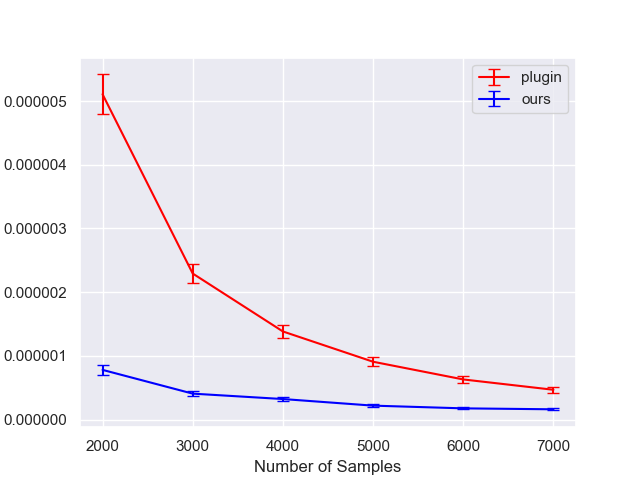
\includegraphics[width=\textwidth]{mse_estimator_100_bins.png}
%          \caption{Mean-squared errors of estimates.
%          \pl{s/ours/canceling}
%          \pl{Number of samples of what - relate to notation in text}
%          \pl{label y-axis}
%          }
%          \label{fig:mse_estimators}
%      \end{subfigure}
%      \hfill
%      \begin{subfigure}[b]{0.45\textwidth}
%          \centering
%          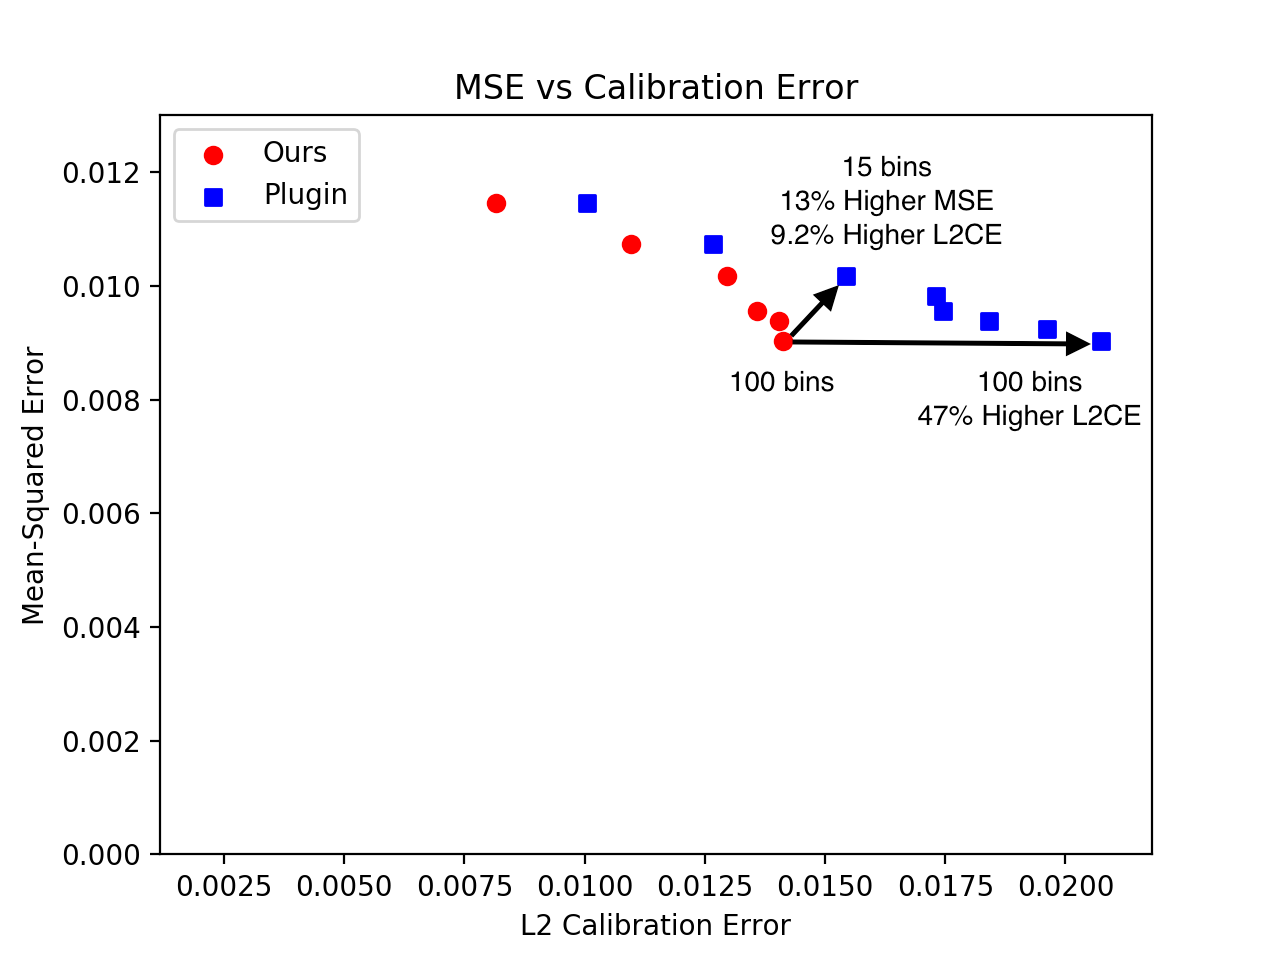
\includegraphics[width=\textwidth]{mse_vs_verified_error_plugin_vs_ours.png}
%          \caption{Brier score vs calibration error.
%          \pl{be consistent with MSE/Brier}
%          \pl{make text larger by reducing the xrange and yrange}
%          }
%          \label{fig:mse_vs_ce_estimators}
%      \end{subfigure}
%   \caption{
%     (\textbf{Left}) Mean-squared errors of cancelling and plugin estimators on a recalibrated VGG-net model on CIFAR-10 with $90\%$ confidence intervals (lower values better). Our estimator is closer to the ground truth \pl{what's ground truth? 0 on the y-axis?}.
%   (\textbf{Right}) Plot of Brier scores against upper bounds \pl{90\% confidence bounds or something?} on the calibration error computed by our estimator and the plugin estimator, when we vary the number of bins $B$. For a given calibration error, our estimator enables us to choose models with a better Brier score. If we want a model with $\ell_2$ calibration error less than 0.015, the cancelling estimator tells us we can confidently use 100 bins, while relying on the plugin estimator only lets us use 15 bins and incurs a 13\% higher Brier score.
%   \pl{I find it awkward that you have MSE (which is squared) plotted against calibration error (non-squared);
%   can we just make it RMSE instead?
%   }
% }
%   \label{fig:mse_estimators_bins}
% \end{figure}

% This means that our estimator has a substantially better dependency on the number of outputs of the model.

% \begin{corollary}
% \label{cor:final-ours}
% Using our estimator $\hat{E}$, if $n = \Theta(kb + \frac{\sqrt{b}}{\epsilon^2})$ ignoring $\log$ factors, we can check if $|{E^*} | \leq \epsilon$ with significance and power $\delta$, and constant effect size $r$. 
% \end{corollary}
